\section{Approach}

%\subsection{Approach Overview}

%In \tool, we have three main steps to do the fault localization. We want to introduce them as follow:

%{\bf Step 1. Data Preprocess.} \tool accepts the java project with all the related test cases as the input for the whole tool. In this step, \tool firstly preprocesses the input into features and graphs in three main directions. And then \tool groups these features and graphs into two big sets for statement-level and method-level fault localization. \tool generates features include: 1) Method content (sequence of sub-tokens); 2) Abstract Syntax Tree (whole method); 3) Most similar buggy method; 4) Code coverage information; 5) Sub-AST (single statement); 6) Variables. \tool generates graphs include: 1) Stack traces; 2) execution path (method level); 3) execution path (statement level); 4) Co-change relationship (method level); 5) Co-change relationship (statement level); 6) Program Dependency Graph (PDG). After having these features, we group the feature 1), 2), and 3) with graphs 1), 2), and 4) as one set for the method-level fault localization usage while we group the rest features and graphs as one set for the statement-level fault localization.

%{\bf Step 2. Feature Representation Learning} In this step, \tool uses different technologies to combine and learn the representations from the features and graphs generated in the last step. 

%For the method-level, \tool collects the stack traces with the depth of 10 with directional edges $E_m^s$ and expands it by adding the execution path and co-change relationships. As for the execution path, \tool starts to find them from the stack traces with the depth of 10 and collects all the methods within ten steps from the crash position in the stack trace. \tool adds these methods by adding a new type of directional edge $E_m^e$ to the stack trace. As for the co-change relationships, \tool collects all co-change information from the repository commit history and adds them to the stack trace with the new type of non-directional edges $E^c$. If a set of methods $M$ has been changed together in previous commits in the repository, \tool regards them as the co-change information. There will be one non-directional edge $E^c$ between every two methods in this set. Because the stack trace graph is a directional graph, to add them to the stack trace graph, we make the non-directional edge $E^c$ become a two-directional edge $E_m^c$ (e.g.$method_A -> method_B$ and $method_B -> method_A$). After having the combined graph $G_m$, for each node, \tool uses RNN model \cite{cho2014learning} to learn the representation of the method content and uses the tree-based model TreeCaps \cite{bui2021treecaps} to learn the representation of the AST and the most similar buggy method. 

%Similar to the method-level, on the statement-level, \tool uses TreeCaps to learn the representation for the sub-AST as one of the node features. And \tool uses the PDG as the base graph and adds the co-change relationship and execution path to build the combined graph $G_s$ in the same way as the method-level. The different features are the code coverage information and variables. For the code coverage information, \tool collects the test cases running results for a statement. If the test case $t_i$ passes the statement, \tool uses $1$ to represent the code coverage information $c_i$ for the test case $t_i$ while \tool uses $0$ to represent $c_i$ when the test case $t_i$ does not pass the statement. By collecting them together, \tool has the code coverage information feature as $<c_1, c_2, ..., c_i>$. And for the variables, \tool collects all variables $v$ that appear in the statement, and for each variable, \tool uses the variable name and type to represent it. By linking these variables as a sequence, \tool uses the RNN model to learn the representation for the variable feature.

%{\bf Step 3. Multi-tasking Fault Localization} After having the feature representations from the last step, \tool uses a multi-tasking framework to do the fault localization. In the framework, there are two tasks: method-level fault localization and method-level fault localization. Among them, statement-level fault localization is the primary goal for the multi-tasking framework.

%For the method-level fault localization, \tool uses the GCN model \cite{kipf2016semi} to do the binary classification $C_m$ for each node based on the combined graph $G_m$. If the method is faulty, the GCN model will classify the node as $1$ while the GCN model classifies the node to $0$ when the method is non-faulty. Like the statement level, \tool uses the other GCN model to classify $C_s$ on the statement level based on the combined graph $G_s$.

%When doing the training, \tool learns the classification on both method-level and state-level and does the soft parameter sharing between the two models to make these two GCN models learn more features from both levels. But when making the prediction, because the statement-level fault localization is the primary goal, \tool only picks the statement-level fault localization results as the final results. Thus, \tool regards all the statements marked as faulty as the model output statement set, which contains the statements predicted to be fixed together in this fault.

%\begin{figure*}[t]
%	\centering
%	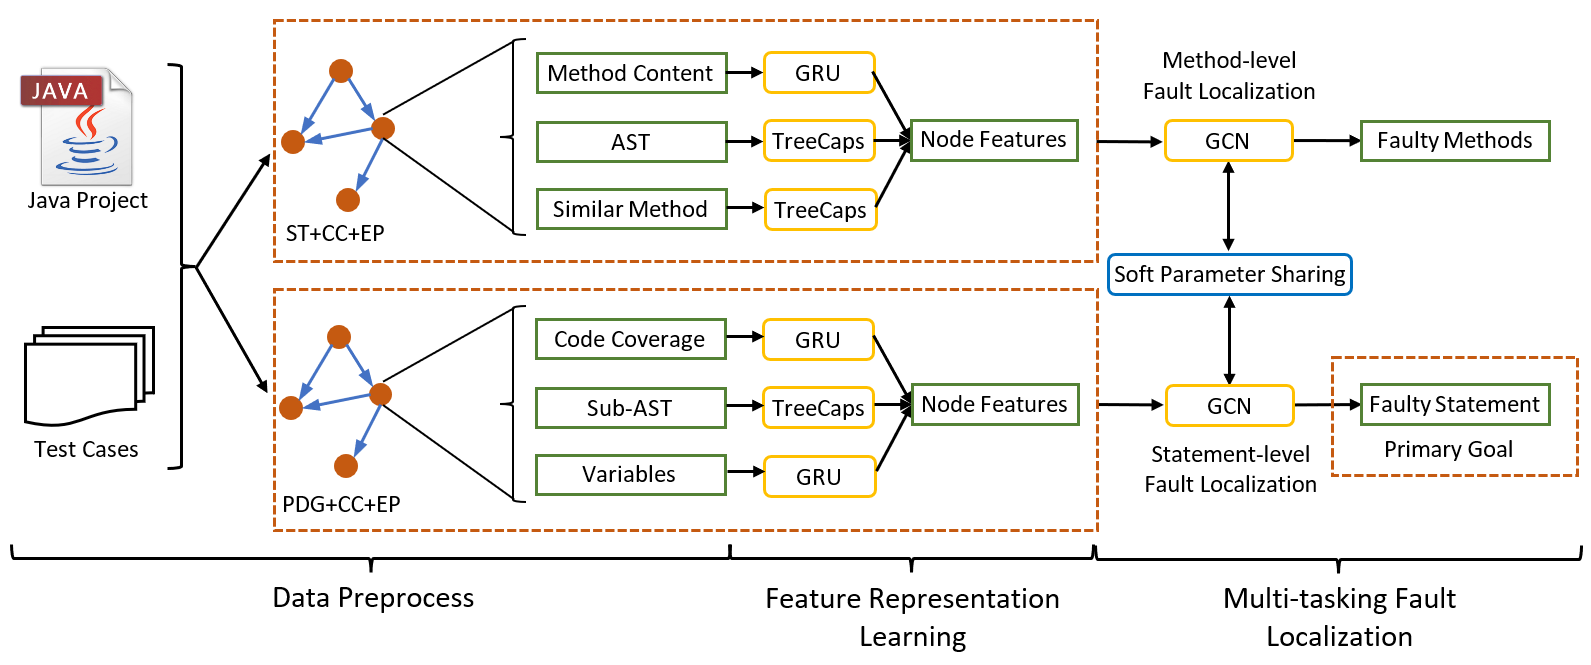
\includegraphics[width=6.5in]{graphs/overview.png}
%	\caption{{\tool}'s Architecture}
%	\label{overview}
%\end{figure*}

%\section{Feature Extraction}

The first step of \tool is to preprocess the input data into the suitable format and group them into statement and method two levels. So the input of this step is the \tool input, including the java project that needs to do the fault localization with the commit history and the relevant test cases for the project. And the output of this step is two groups of graphs with node features for statement-level and method-level.

Specifically, \tool extract the features from two levels: the method-level and statement-level feature extraction.

\begin{figure}[t]
	\centering
	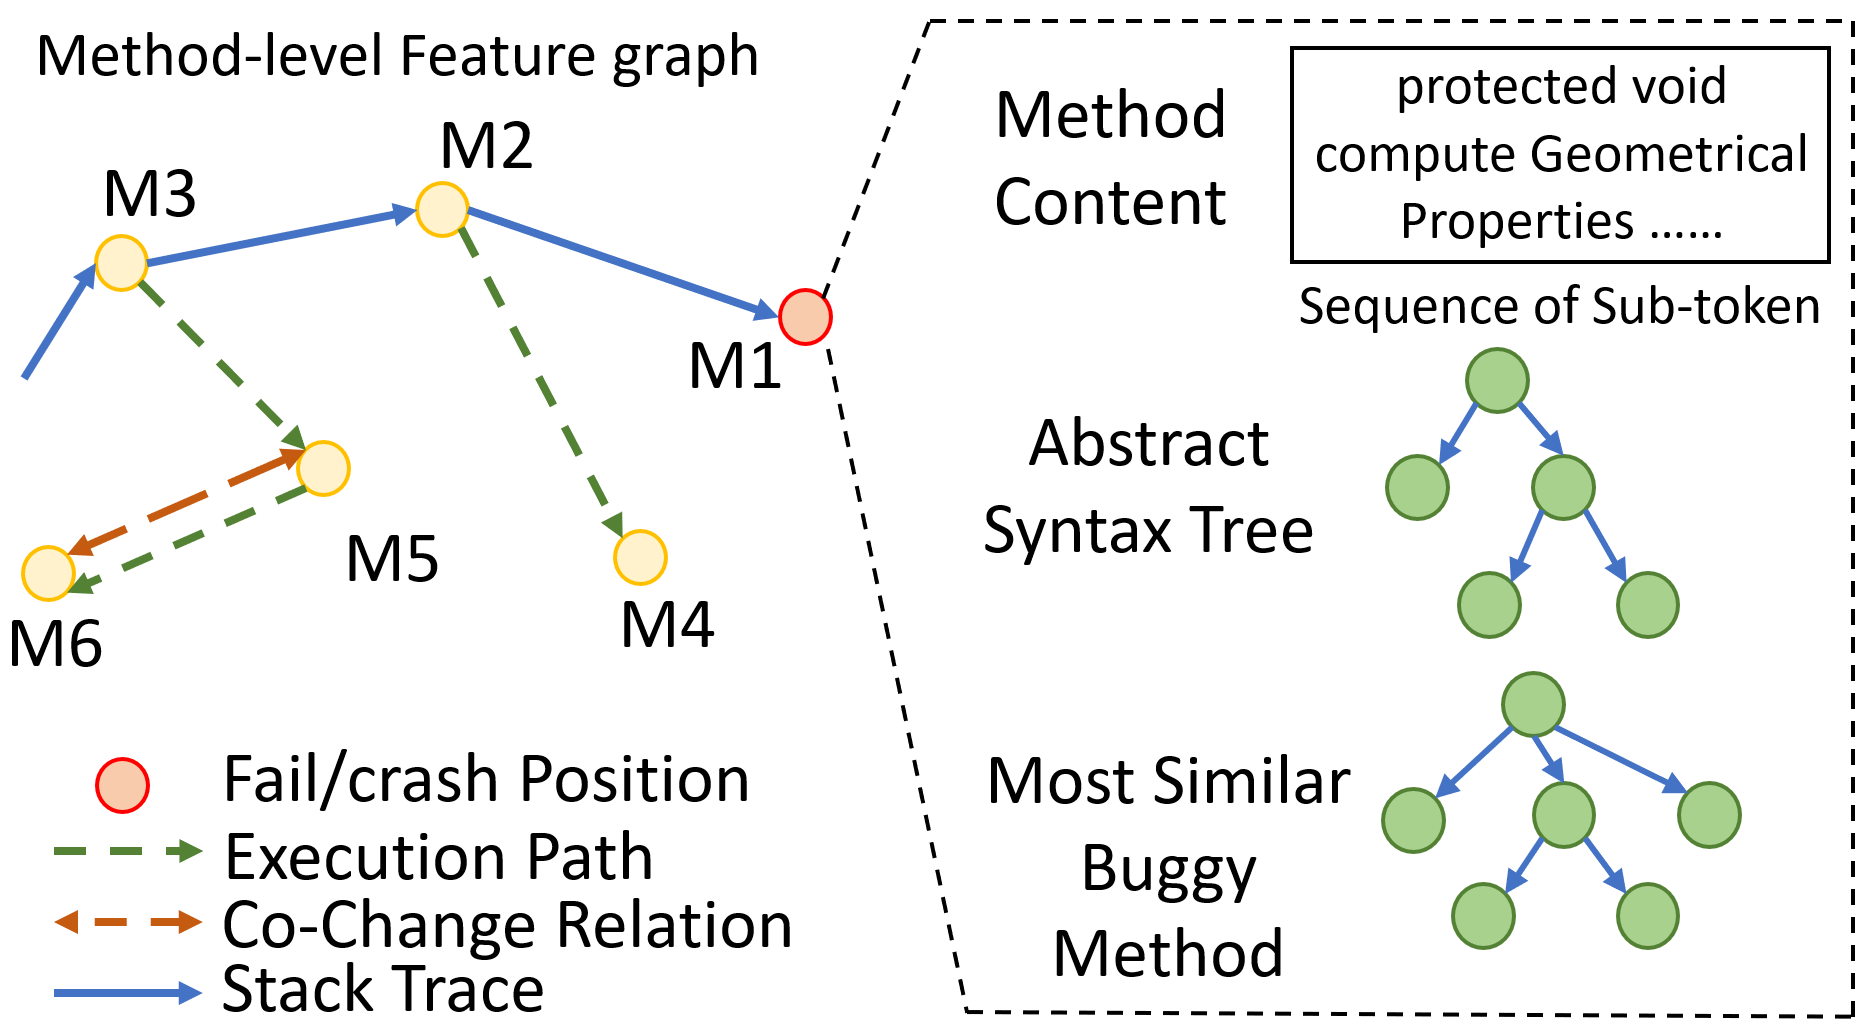
\includegraphics[width=3in]{graphs/step-1-method.png}
	\caption{Method-level Feature Extraction}
	\label{method-level-feature-extraction}
\end{figure}

\subsection{Method-level Feature Extraction}
For the method level, \tool uses the method as the basic unit. And for each method, \tool extracts three key features, including the method content, abstract syntax tree (AST), and the most similar buggy method. 1> For the method content, \tool collect the source code of each method $M$ and link each statement $S_m$ one by one in $M$ as a sequence $Seq_m$ to represent the method content. \tool removes all special characters and uses CamelCase to break down the tokens in the sequence into sub-tokens to reduce the influence of biases. For example, in the Figure \ref{method-level-feature-extraction}, the method content feature in the method $M1$ shows the extracted sequence of sub-tokens $protected void compute ......$. The source code is listed on the input of the Figure \ref{statement-level-feature-extraction}. 2> As for the AST, \tool generates abstract syntax tree $Tree_m$ for each method $M$ by using JDT package \cite{JDT}. The generated AST looks like the example shown on the abstract syntax tree feature in Figure \ref{method-level-feature-extraction}. 3> When extracting the most similar buggy method feature, \tool breaks down the methods into the sequence of sub-tokens just like the method content feature. It then uses GloVe \cite{pennington2014glove} to learn the embedding for each sub-token and replace the sub-tokens with the embedding vectors. After this, \tool calculates the cosine similarity between the current method $m$ and all other buggy methods in the commit history (before the current bug) to find the most similar buggy method $m_b$. For this buggy method, \tool also uses the JDT package to generate the AST for $m_b$. The most similar buggy method feature in Figure \ref{method-level-feature-extraction} shows a possible example for it.

After having these three features for each method, \tool uses three kinds of edges to link them as a graph. First of all, \tool runs test cases for the project. If a test case $t_i$ failed, \tool collect the stack trace for the test case $t_i$. Because the stack trace is sometimes too long, using the crashed position as the root, \tool only picks part of the stack trace $st_i$ with the depth of ten in consideration. It means that on the stack trace $st_i$, there are at most ten methods include $m_1, m_2, ..., m_{10}$ where $m_1$ is the crashed position. For every two method $m_j$ and $m_{j+1}$ among these methods, $m_{j+1}$ calls the $m_j$ in the stack trace. The edge $E_m^s$ direction in it is always from $m_{j+1}$ point to $m_j$. For example, in the Figure \ref{method-level-feature-extraction}, the crashed method is $M1$ and the blue solid edges are the stack trace $st_i$. The figure shows that in the stack trace, $M3$ comes out before $M2$ and $M2$ comes out before $M1$. The second type of edge is the execution path. By using each method $m_j$ in the stack trace $st_i$ as the root method, \tool expands the stack trace $st_i$ by adding the executed methods into the graph. The direction of the execution edges $E_m^e$ is also the same as the call direction. Also, because sometimes the execution path may be very long for a method, we only keep the methods $m_k$ within ten steps from the crashed position $m_1$ that means in the graph, from node $m_k$ to $m_1$, the steps are no more than ten (when counting the steps, \tool ignore the edge direction). The green dotted line in Figure \ref{method-level-feature-extraction} shows an example for this type of edge. With the Figure \ref{method-level-feature-extraction}, the green dotted line reflects the relationship that when running the test case $t_i$ on $M2$, it also executes the method $M4$ based on the method call. And then, it executing the $M3$, it executes the method $M5$, and within $M5$, it also executes method $M6$ based on the method calls inside the methods. The third type of edge is the co-change relation. For this,  \tool collects all commit history from the input java project. If more than one method has changed in one commit, we mark it as a co-change. The co-change contains all the methods that changed together in this commit. To add the co-change relation as one type of edge, \tool makes the co-change relation become a two-directional edge $E_m^c$ (e.g. The orange edge between $M5->M6$ and $M6->M5$ in the Figure \ref{method-level-feature-extraction}).
%
%\begin{itemize}%
%	\item Graph: 
%	\begin{itemize}
%		\item Stack Trace: \tool runs test cases for the project. If a test case $t_i$ failed, \tool collect the stack trace for the test case $t_i$. Because the stack trace may be very bug, by using the crashed position as the root, \tool pick part of the stack trace $st_i$ with the depth of ten. It means that on the stack trace $st_i$, there are ten methods include $m_1, m_2, ..., m_{10}$ where $m_1$ is the crashed position and for every two method $m_j$ and $m_{j+1}$ among them, $m_{j+1}$ calls the $m_j$ in the stack trace. The edge $E_m^s$ direction in it is always from $m_{j+1}$ point to $m_j$ \tool uses $st_i$ as the base graph and the relationship information in $st_i$ is the dynamic information. 
%		\item Execution Path: As for the failed test case $t_i$, \tool also analyzes the execution path. By using each method $m_j$ in the stack trace $st_i$ as the root method, \tool expands the stack trace $st_i$ by adding the executed methods into the graph. The direction of the execution edges $E_m^e$ is also the same as the call direction. Also, because sometimes the execution path may be very long for a method, we only keep the methods $m_k$ within ten steps from the crashed position $m_1$ that means in the graph, from node $m_k$ to $m_1$, the steps are no more than ten (when counting the steps, \tool ignore the edge direction). The added execution information here is the dynamic edge.
%		\item Co-change Information: \tool collects all commit history of the input java project. If more than one java method has changed in one commit, we mark it as a co-change. The co-change contains all the methods that changed together in this commit. Because the co-change does not have the direction, there is one non-directional edge $E^c$ between every two methods in this co-change to represent the co-change relationship. In order to add the co-change relationship into the stack trace, \tool makes the non-directional edge $E^c$ become a two-directional edge $E_m^c$ (e.g.$method_A -> method_B$ and $method_B -> method_A$). This type of edge is the static edge.
%	\end{itemize}
%	\item Node Features: 
%	\begin{itemize}
%		\item Method Content: \tool collect the source code of each method $M$ and link each statement $S_m$ one by one in $M$ as a sequence $Seq_m$ to represent the method content. \tool removes all special characters and uses CamelCase to break down the tokens in the sequence into sub-tokens to reduce the influence of biases. For example, the $setTagAsStrict$ can be break down into $set, Tag, As,$ and $Strict$. The processed sequence of sub-tokens $Seq^p_m$ is used to represent the method content in \tool. This feature is one of the static features that \tool collects from the source code to represent the method.
%		\item Method Structure: \tool generates abstract syntax tree $Tree_m$ for each method $M$ by using JDT package \cite{JDT}. Each tree $Tree_m$ represent the structure of the relevant method $m$. This is one of the static feature that \tool collect from the source code to represent the method.
		%\item Similar Buggy Method: \tool breaks down the methods into the sequence of sub-tokens just like method content feature and then uses GloVe \cite{pennington2014glove} to learn the embedding for each sub-token and replace the sub-tokens with the embedding vectors. After this, \tool calculate the cosine similarity between the current method $m$ and all other buggy methods in the commit history (before current bug) to find the most similar buggy method $m_b$. This is one of the static feature that \tool collect from the source code to represent the method.
%	\end{itemize}	
%\end{itemize} 


\begin{figure}[t]
	\centering
	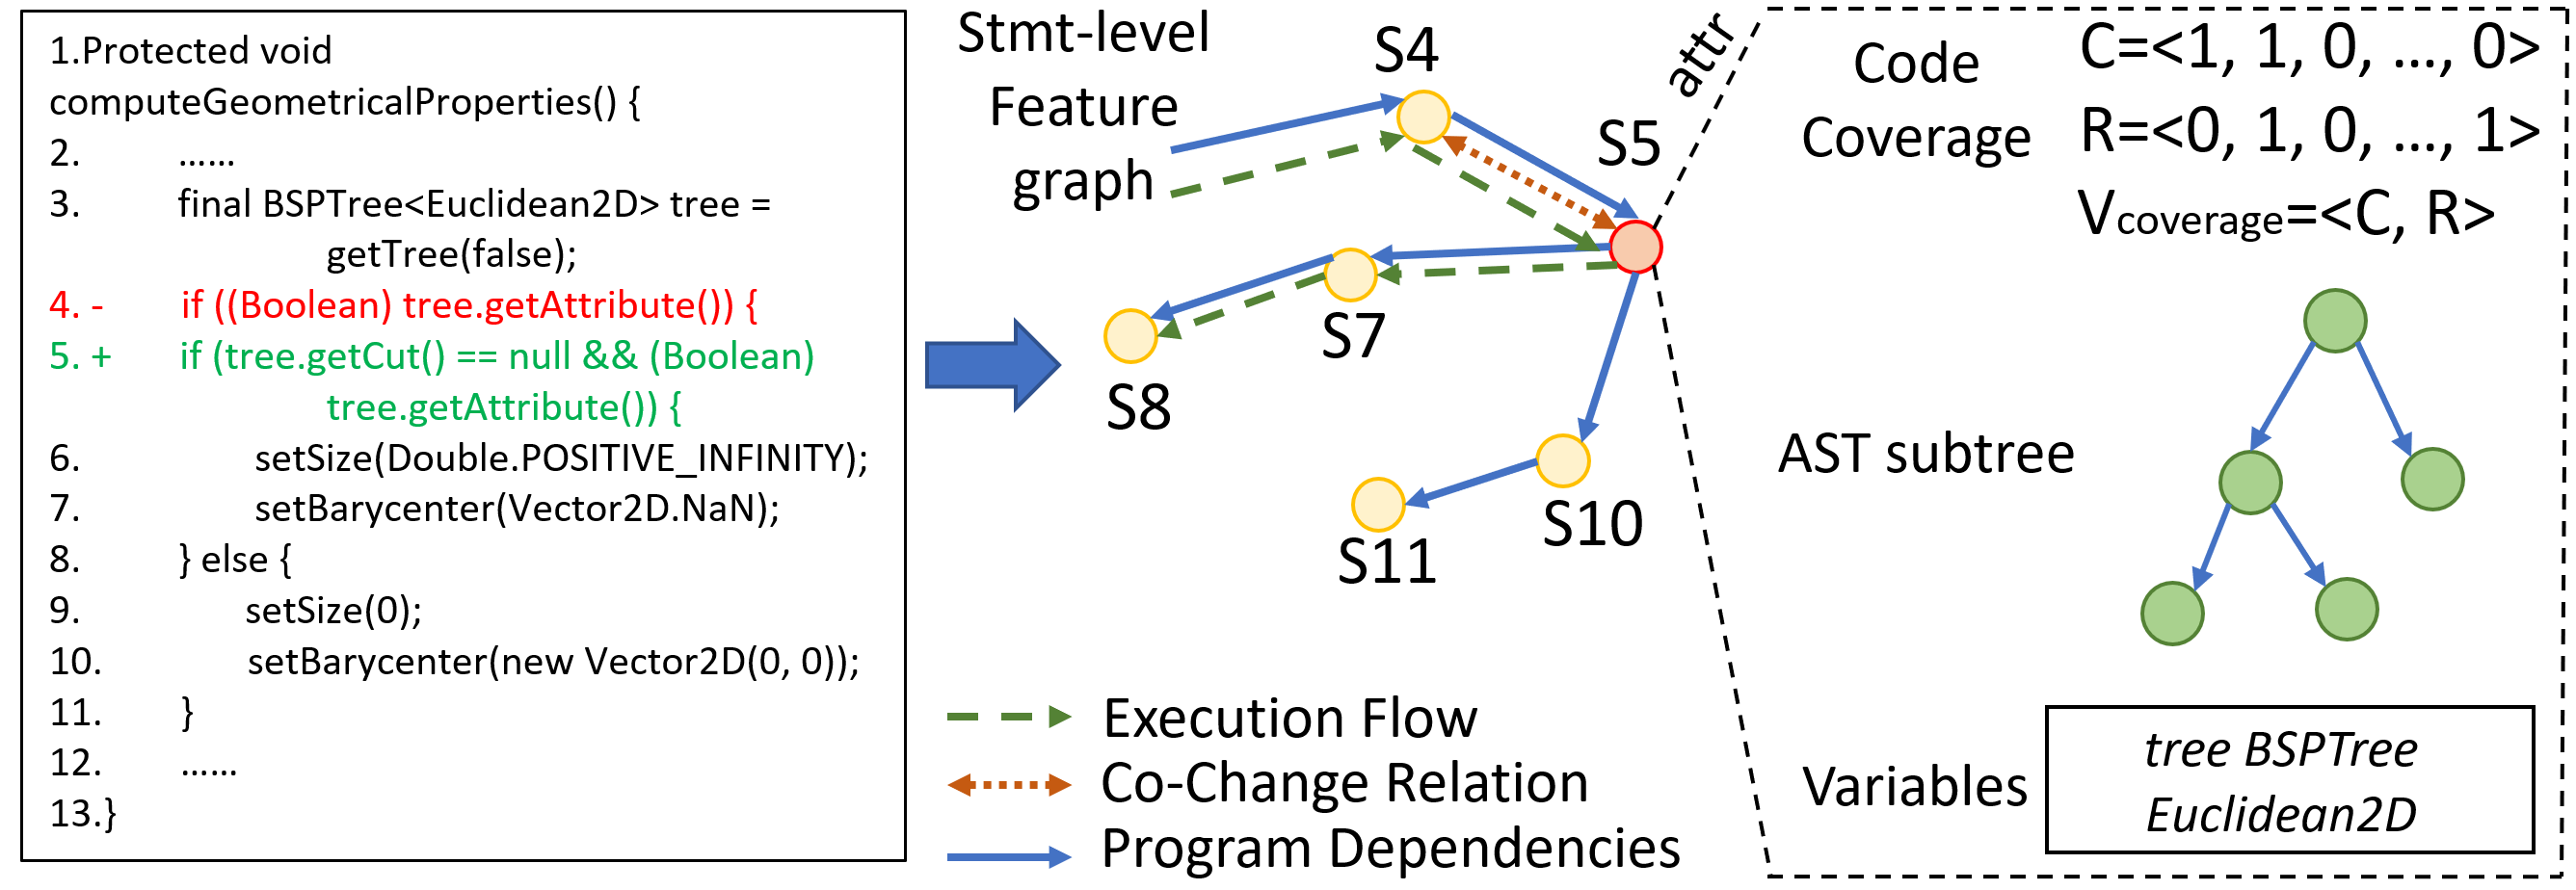
\includegraphics[width=3.4in]{graphs/step-1-statement.png}
	\caption{Statement-level Feature Extraction}
	\label{statement-level-feature-extraction}
\end{figure}

\subsection{Statement-level Feature Extraction}

For the statement level,  \tool uses the statement as the basic unit. And for each statement, \tool extracts three key features, including the code coverage information, sub-AST, and variables to represent the statement. 1> As for the code coverage information, \tool runs the relevant test cases for the input project. For the test case $t_i$, if it passes the statement $s_i$, \tool uses $c_i = 1$ to represent it while if it does not pass the statement $s_i$, \tool uses $c_i = 0$ to represent it. By linking all $c_i$ together, \tool can get $C = <c_1, c_2, ..., c_i>$. Also, \tool uses $r_i = 1$ to represent the the condition $passed$ and uses $r_i = 0$ to represent the condition $failed$ for the test case $t_i$ . By linking all $r_i$ together, \tool can get $R = <r_1, r_2, ..., r_i>$. By concatenate $C$ and $R$, \tool extract the code coverage information feature by $V_{coverage} = <c_1, c_2, ..., c_i, r_1, r_2, ..., r_i>$. The code coverage information feature in Figure \ref{statement-level-feature-extraction} shows an example of it. 2> For the sub-AST, it is very similar to the method level. By using JDT package, \tool can extract the AST for the whole method. And then, \tool searches for the nodes that appears in the statement. By collecting all these nodes and the edges between then, \tool can extract the sub-AST for the statement. 3> For the variables feature, for each statement, \tool collects all the variables $V$ that appeared in it and for each variable $v$ in $V$, \tool uses the $(variable_name variable_type)$ to represent it. Then \tool links all variables $V$ together with $,$ as a sequence $Seq_s$ as one of the static feature that \tool collect from the source code to represent the statement. For example, in Figure \ref{statement-level-feature-extraction}, \tool goes through the statement at $line 5$ in the input method and finds that only one variable $tree$ appears in the statement at $line 5$. So the variable feature here should be like $variable_name variable_type$ where $variable_name$ is $tree$ and $variable_type$ is $BSPTree Euclidean2D$.

With these three features, similar to the method-level, \tool builds three types of edges to link the statements together as a graph. The first type of edge is the program dependency edge (PD). \tool builds the PD by using the tool soot \cite{soot} for the method $m$. For example, in Figure \ref{statement-level-feature-extraction}, the blue edges are the PD edges and they show that in method $m$, statement at $line 4$ controls the statement at $line 5$. And statement at $line 5$ can control the statements at $line 7-8$ and the statements at $line 10-11$. The second type of edge that \tool extracts is the execution flow $E_s^e$. The execution flow is the order that the failed test case $t_i$ went through in the method $m$. For example, the green dotted edges are the execution flow. Within it, we can see that the test case executes $S7-S8$ but did not go through $S10-S11$. Even though in the PD, $S5$ is linked by $S10-S11$. It means that when running the test case $t_i$, it will not pass the $S10$ and $S11$ because of the if checking in $S5$. The last type of edge $E_s^c$ is the co-change relation in the statement level. \tool collects the co-change information for the commit about the statements that changed together before in the current method $m$ and one commit. In Figure \ref{statement-level-feature-extraction}, the commit history shows that $S4$ and $S5$ used to be changed together before. Hence, there is an orange edge that represents the co-change relation between $S4$ and $S5$.


%\begin{itemize}
%	\item Graph: 
%	\begin{itemize}
	%	\item Program Dependency Graph (PDG): \tool builds the PDG by using the tool soot \cite{soot} for the method $m$ that contains the statements that \tool want to analyze. \tool uses the generated PDG as the base graph. Within this graph, there are two types of edges including data dependency and control dependency. Both of these two types of edges are the static edges.
	%	\item Execution Path: \tool collects the execution path of the failed test case $t_i$ within the method $m$ and adds them into the PDG by adding a new type of edge $E_s^e$. The new edge direction is the same as the execution order. This type of edge is the dynamic edge.
%		\item Co-change Information: Similar to the method-level, \tool collects the co-change information for the commit about the statements that changed together before in one commit and the current method $m$. As for adding the co-change information into the PDG, \tool also creates the two-directional edge $E_s^c$ similar to the method level. This type of edge is the static edge.
%	\end{itemize}
%	\item Node Features: 
%	\begin{itemize}
	%	\item Code Coverage Information: \tool runs the relevant test cases for the input java project. For the test case $t_i$, if it passes the statement $s_i$, \tool uses $c_i = 1$ to represent it while if it does not pass the statement $s_i$, \tool uses $c_i = 0$ to represent it. By linking all $c_i$ together as $C = <c_1, c_2, ..., c_i>$, $C$ is considered by \tool as one of the dynamic feature.
	%	\item Statement Structure: Similar to the method-level, \tool generates a sub abstract syntax tree $Tree_s$ for each statement $S$ by using JDT \cite{} package. Each tree $Tree_s$ represent the structure of the relevant statement $s$. This feature is one of the static features that \tool collects from the source code to represent the statement.
	%	\item Variables: For each statement, \tool collects all the variables $V$ that appeared in it and for each variable $v$ in $V$, \tool uses the $(variable_name variable_type)$ to represent it. Then \tool links all variables $V$ together with $,$ as a sequence $Seq_s$ as one of the static feature that \tool collect from the source code to represent the statement. For example, the variables in the statement in line 3 in Figure \ref{fig:motiv} include $root$ and $sourceMap$. \tool generates the feature for them as $root Node, sourceMap SourceMap$ where $root$ and $sourceMap$ are the names and $Node$ and $SourceMap$ are the types.
%	\end{itemize}	
%\end{itemize} 

\subsection{Step 2. Feature Representation Learning.}

In this step, \tool aims to learn the node feature embeddings based on the graphs with the node features generated from step 1. So the input of this step is the method-level and statement-level graphs, and the expected output is the node embedding vectors for each node in each graph.

To be more in detail, \tool generates the node feature embedding as follow:

{\bf As for the Method-Level:}
\begin{itemize}
	\item Method Content: \tool has the processed sequence of sub-tokens $Seq^p_m$ from the last step. In this step, \tool uses the GloVe \cite{pennington2014glove} to learn the sub-token embedding and then replace each sub-token with the embedding vector generated from GloVe. After the replacement, \tool has a sequence of vector $Seq^{pe}_m$ and then uses a GRU layer \cite{cho2014learning} to learn the embedding vector $vec_{mc}$ for the method content. 
	
	\item Method Structure: \tool has the generated AST $Tree_m$ from the last step. In this step, \tool also firstly uses the GloVe to vectorize the AST and then uses a deep learning-based model TreeCaps \cite{bui2021treecaps} to learn the embedding vector $vec^{ms}$.
	
	\item Similar Buggy Method: \tool has the most similar buggy method $m_b$ from the last step. In this step, \tool has the same process as the method structure feature by using the GloVe and TreeCaps to learn the embedding vector $vec^{sbm}$.
\end{itemize}

{\bf As for the Statement-Level:}
\begin{itemize}
	\item Code Coverage Information: \tool has the code coverage information $C = <c_1, c_2, ..., c_i>$ from last step. In this step, \tool does not make any changes and directly regard $C$ as the embedding vector $vec_{cci}$ for the code coverage information.
	
	\item Statement Structure: \tool has the generated sub-AST $Tree_s$ from the last step. In this step, \tool does a similar process as the method-level by firstly using the GloVe to vectorize the AST and then using a deep learning-based model TreeCaps to learn the embedding vector $vec^{ss}$.
	
	\item Variables: \tool has the variable sequence with variable types $Seq_s$ from the last step. In this step, \tool uses the GloVe to learn the token (here can be the variable name and variable type) embedding and then replace each token with the embedding vector generated from GloVe. And then, \tool uses one GRU layer to learn the embedding vector $vec_{v}$ for the whole variable information sequence $Seq_s$
\end{itemize}

After having the six embedding vectors mentioned above, \tool uses six fully connected layers to standardize each embedding vector's length to $l/3$ (Here l/3 is an integer). And then, for both method-level and statement-level, \tool concatenate three feature embedding vector into one vector $vec_{m}$ or $vec_{s}$ for the method-level or statement-level with the length of $l$. In this case, for both method-level and statement-level, \tool all has a combined graph $G_m$ or $G_s$ with the node embedding vector $vec_{m}$ or $vec_{s}$. It is the input for the next step.

\section{Dual-Learning Fault Localization}

\begin{figure}[t]
	\centering
	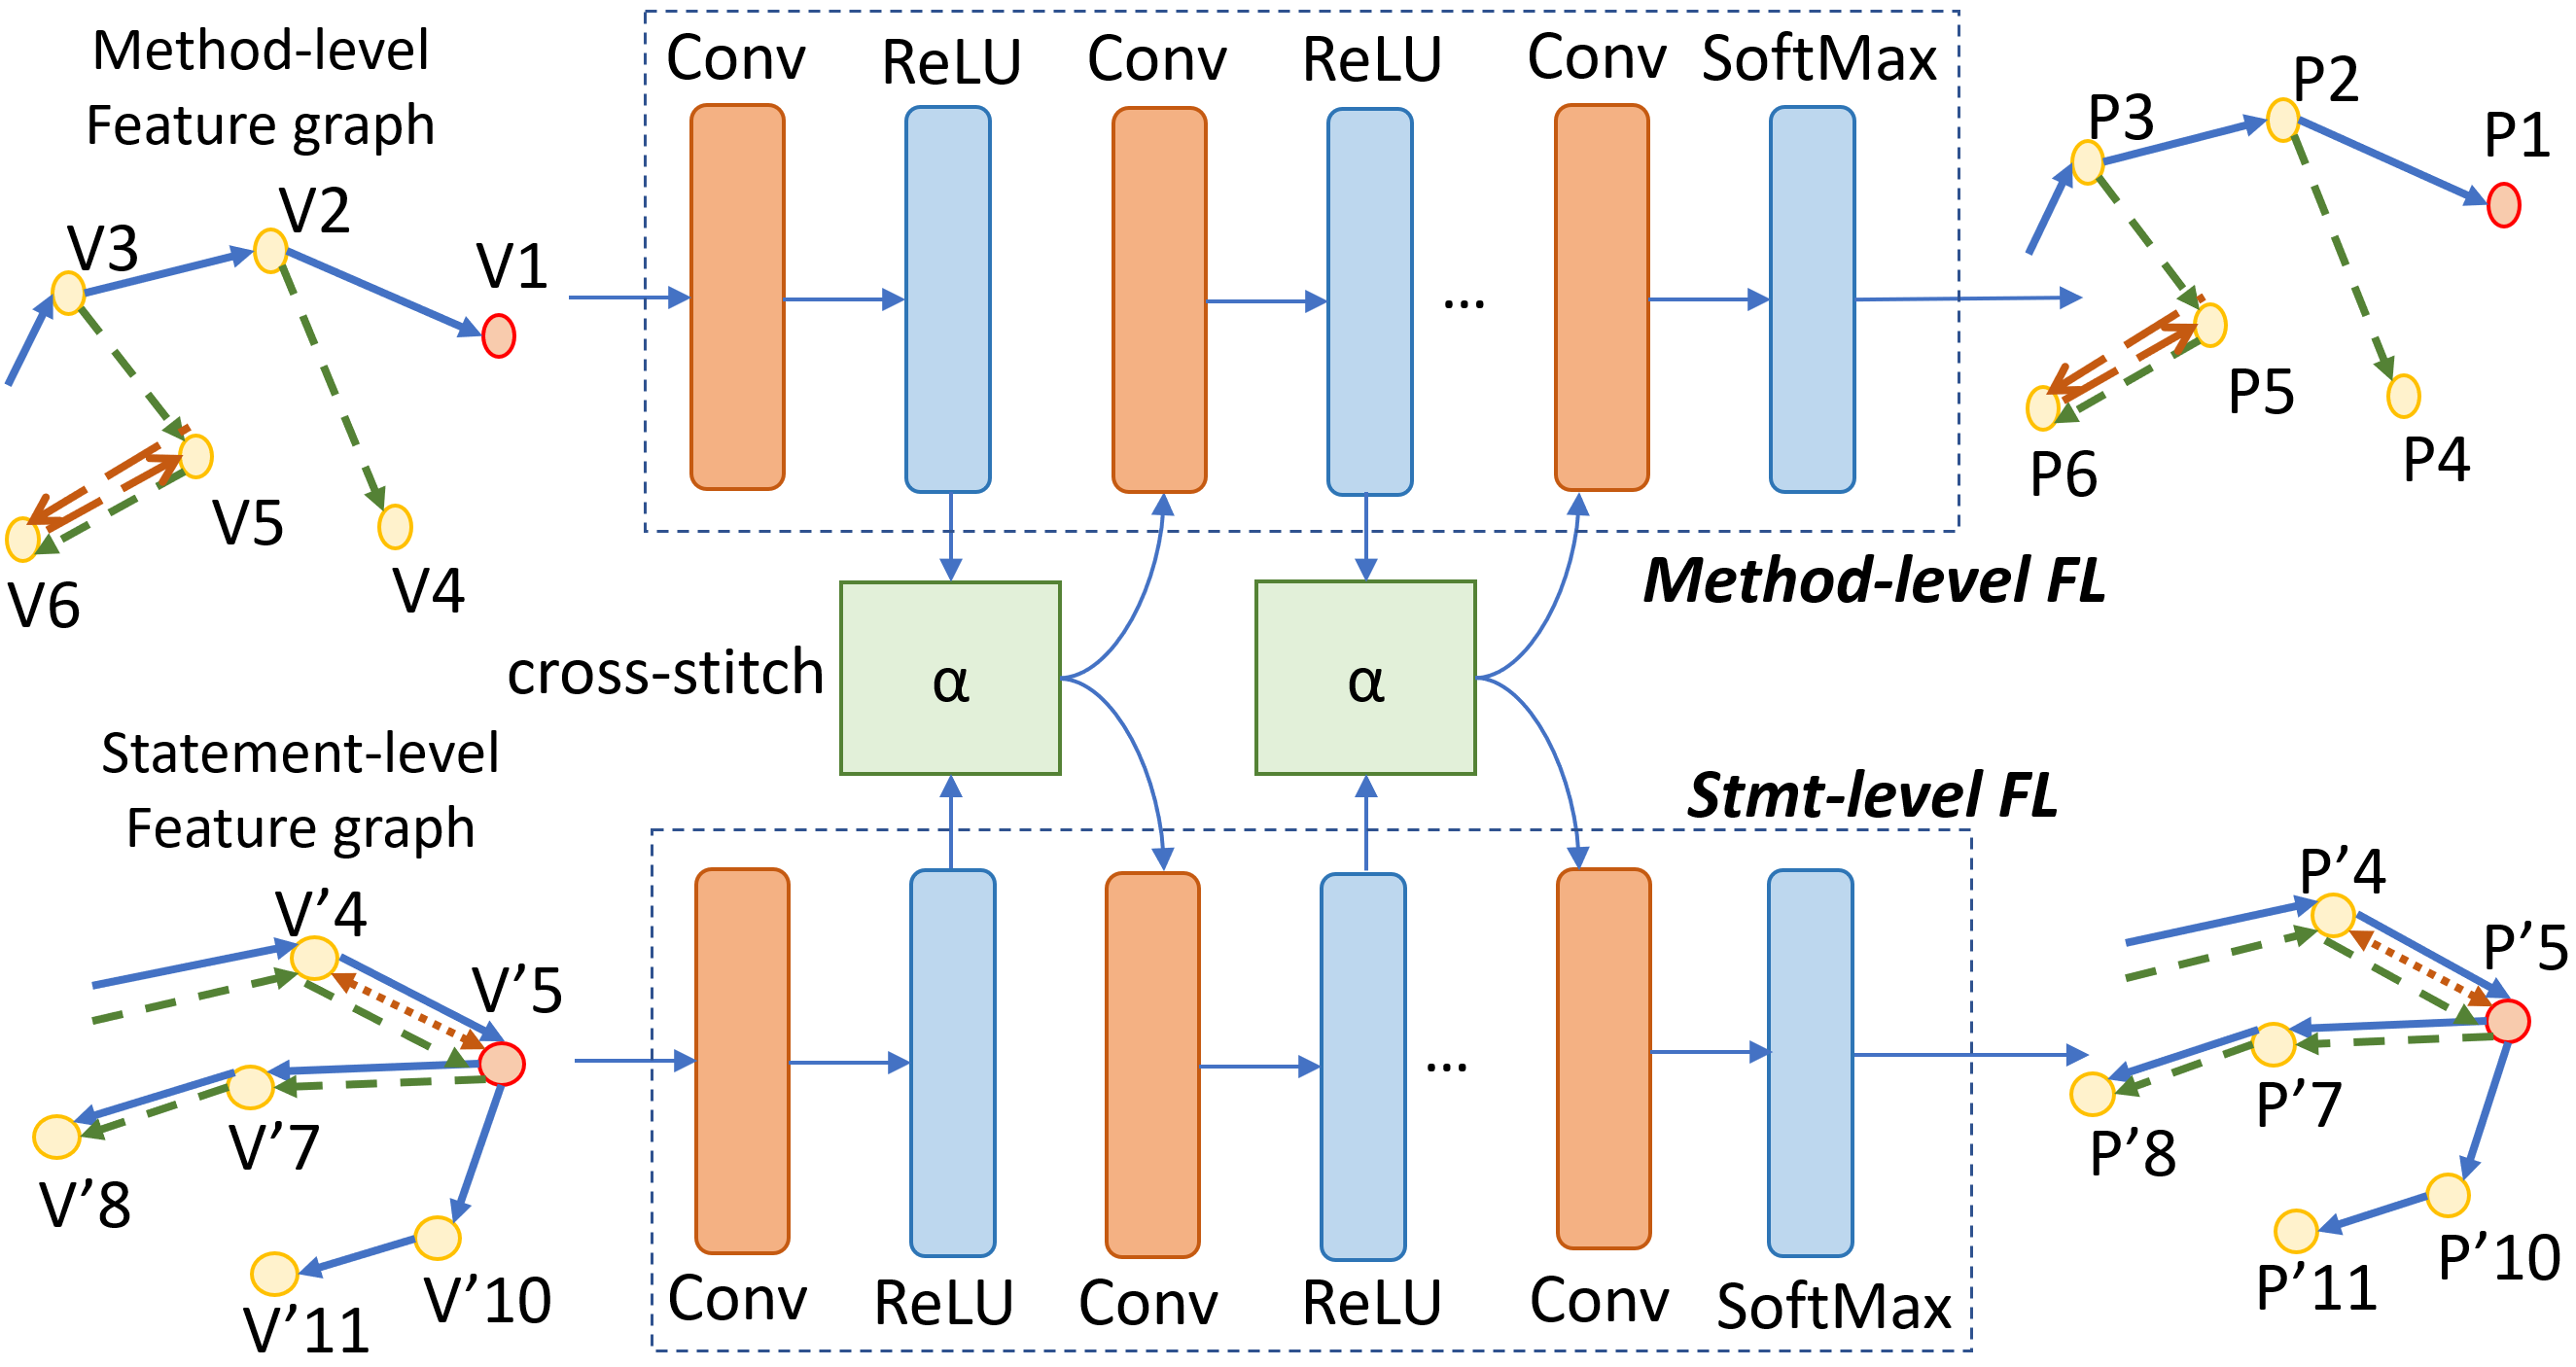
\includegraphics[width=3.4in]{graphs/dual-learning.png}
	\caption{Dual-Learning Fault Localization}
	\label{dual-learning}
\end{figure}

\begin{figure}[t]
	\centering
	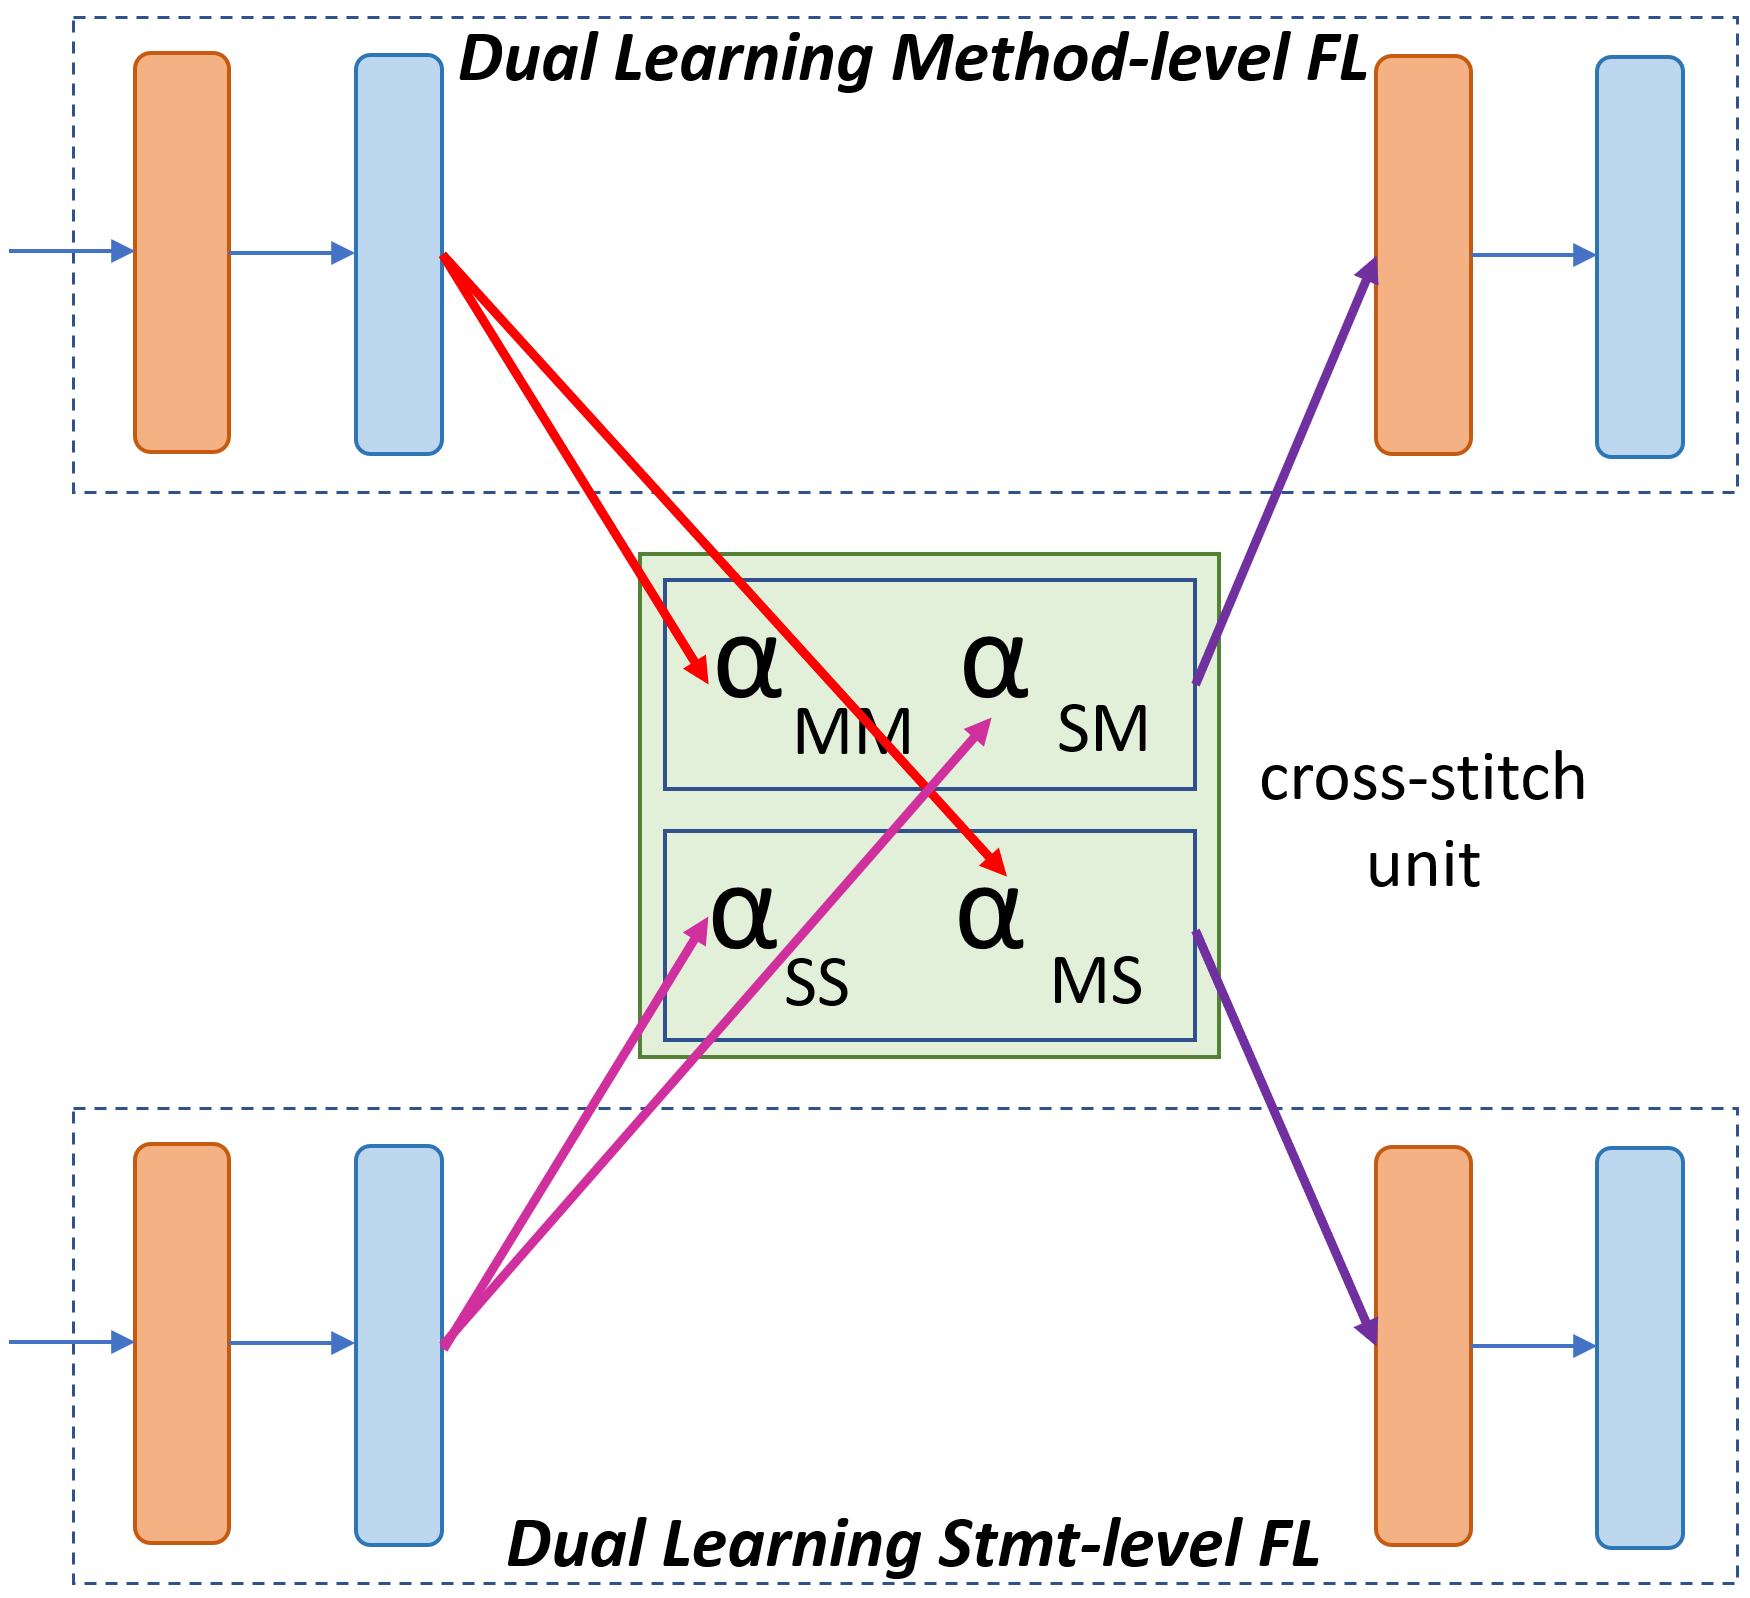
\includegraphics[width=2in]{graphs/cross-stitch.png}
	\caption{Dual Learning via Cross-stitch Unit}
	\label{cross-stitch}
\end{figure}

This section explains our dual learning scheme in step 3 (illustrated
in Figures~\ref{dual-learning} and~\ref{cross-stitch}). The input of
this step includes two feature graphs $G_M$ and $G_S$ for the method
and statement levels. Each node in each feature graph is a vector
computed for a method or a statement (explained in
Section~\ref{feature-learning:sec}). The output is the output graphs
for methods and statements. For the training process, each node in an
output graph has a buggy or non-buggy label.  For the prediction, each
node in an output graph will be predicted as buggy or non-buggy.

%After having the vectorized graph $G_m$ and $G_s$ for both the method-level and the statement-level features,

%in this step, \tool applies a dual learning fault localization model to extract the fault locations. So there are two main tasks in this step, including the method-level fault localization and the statement-level fault localization. So the input for this step is the two graphs $G_m$ and $G_s$, and the expected output is the prediction label for each node in these two graphs from these two tasks.

%Tien
\noindent {\bf Graph Convolution Network (GCN) for FL.} First, {\tool}
has two GCN models~\cite{kipf2016semi}, each for FL at the method and
statement levels. Each GCN model has $n-1$ pairs of a graph
convolution layer (\code{Conv}) and a rectified linear unit
(\code{ReLU}). They are aimed to consume and learn the characteristic
features in the input feature graph. The last pair of each GCN model
is a pair of a graph convolution layer (\code{Conv}) and a softmax
layer (\code{SoftMax}). The \code{SoftMax} layer plays the role of the
classifier on whether a node corresponding to a method or a statement
is labeled as buggy or non-buggy.

\noindent {\bf Dual Learning with Cross-stitch Unit.} In a regular GCN
model, those above pairs of \code{Conv} and \code{ReLU} are connected
to one another. However, to achieve dual learning between method-level
and state\-ment-level FL (\code{methFL} and \code{stmtFL}), we apply a
cross-stitch technique~\cite{misra2016cross} to connect the two GCN
models. The sharing of representations between \code{methFL} and
\code{stmtFL} is modeled by learning a linear combination of the input
features in both feature graphs. At each of the \code{ReLU} layer of
each GCN model (Figure~\ref{cross-stitch}), we aim to learn such a
linear combination of the output from the graph convolution layer
(\code{Conv}) of \code{methFL} and \code{stmtFL} models.

The top sub-network in Figure~\ref{dual-learning} gets direct
supervision from \code{methFL} and indirect supervision (through
cross-stitch units) from \code{stmtFL}~\cite{misra2016cross}.
Cross-stitch units help regularize both tasks \code{methFL} and
\code{stmtFL} by learning and enforcing shared representations by
combining feature maps~\cite{misra2016cross}.


%Tien
%The α values of a cross-stitch unit model linear combinations of
%feature maps. Their initialization in the range [0, 1] is important
%for stable learning, as it ensures that values in the output
%activation map (after cross-stitch unit) are of the same order of
%magnitude as the input values before linear combination.
%-----

\noindent {\bf Formulation.} Let us explain the mathematic foundation
of this scheme. For each pair of the GCN model, the outputs of the
\code{ReLU} layer, called the hidden states, are computed as follows:
\begin{equation}\label{eq:1}
	\hat{A} = D'^{-\frac{1}{2}}A'D'{-\frac{1}{2}}
\end{equation}

\begin{equation}\label{eq:2}
	H_i = \Delta(\hat{A}X_iW_i)
\end{equation}
Where $A'$ is the adjacency matrix of each feature graph; $D'$ is the
degree matrix; $W_i$ is the weight matrix for layer $i$; $X_i$ is the
input for layer $i$; $H_i$ is the hidden state of layer $i$; and
$\Delta$ is the activation function \code{ReLU}. $H_i$ is the output
from the \code{ReLU} layer. In a regular GCN, it is the input of the
next layer of GCN (i.e., the input of \code{Conv}).

In Figures~\ref{dual-learning} and~\ref{cross-stitch}, a cross-stitch
unit is inserted between the \code{ReLU} layer of the previous pair
and the \code{Conv} layer of the next one. The input of the
cross-stitch is the outputs of the two \code{ReLU} layers: $H_M^i$ and
$H_S^i$ (i.e., the hidden states of those layers at \code{methFL} and
\code{stmtFL}). We aim to learn the linear combinations of both inputs
of the cross-stitch unit, which is parameterized using the weights
$\alpha$.

The output of the cross-stitch unit is computed as:
\begin{equation}\label{cross-stitch-formula}
	\begin{bmatrix}
		X_M^{i+1}\\
		X_S^{i+1}
	\end{bmatrix}
        =
        \begin{bmatrix}
		\alpha_{MM} &  \alpha_{MS} \\
		\alpha_{SM} &  \alpha_{SS}
	\end{bmatrix}
	\begin{bmatrix}
		H_M^{i}\\
		H_S^{i}
	\end{bmatrix}
\end{equation}
Where $\alpha$ is the trainable weight matrix; $X_M^{i+1}$ and
$X_S^{i+1}$ are the inputs for the $(i+1)^{th}$ layers of GCN at the
method and statement levels.

$X_M^{i+1}$ and $X_S^{i+1}$ contain the information learned from both
\code{MethFL} and \code{StmtFL}, which helps achieve the main goal for
dual learning to enhance the performance of fault localization on both
levels.

In general, $\alpha$s can be set. If $\alpha_{MS}$ and $\alpha_{MS}$
are set to zeros, the layers are made to be task-specific.  The
$\alpha$ values model linear combinations of feature maps. Their
initialization in the range [0,1] is important for stable learning, as
it ensures that values in the output activation map (after
cross-stitch unit) are of the same order of magnitude as the input
values before linear combination~\cite{misra2016cross}.




%units combine the activations from multiple networks and can be
%trained end-to-end.

%Specifically, \tool firstly builds two separate GCN models \cite{kipf2016semi} for the method-level fault localization and the statement-level fault localization. For the GCN model applied on the method-level, there are $i$ graph convolutional layer $Conv_1, Conv_2, ..., Conv_i$ as shown in Figure \ref{dual-learning} and after each graph convolutional layer $Conv_i$, there is $ReLU$ layer follows it. Considering a graph convolutional layer $Conv_i$ and the following $ReLU$ layer together as one big layer, the GCN model contains $i$ layers in total. The only special case is in the last layer. There is a $SoftMax$ layer following the graph convolutional layer instead of a $RuLU$ layer. Similar to the GCN model applied on the method-level, for the statement-level fault location, there is the other GCN model with $i$ layers. Each layer contains one graph convolutional layer $Conv'_i$ and one $Relu$ layer. And the $SoftMax$ layer replaces the $ReLU$ layer in the last layer of the GCN model.


%To achieve the information sharing between two layers as a dual learning framework, we use the cross-stitch unit \cite{misra2016cross} for help. To be more detailed, for each layer of GCN, it calculates the hidden status using the following formula.





%Where $A'$ is the adjacency matrix; $D'$ is the degree matrix; $W_i$ is the weight matrix for layer $i$; $X_i$ is the input for layer $i$; $H_i$ is the hidden status of layer $i$; and $\Delta$ is the activation function $ReLU$. $H_i$ here is the output from the $ReLU$ layer and will be regarded as the input of the next layer of GCN. The cross-stitch unit is suitable to be added here.

%As seen in Figure \ref{dual-learning}, after the $ReLU$ layers we have $H_i^m$ and $H_i^s$ as the method-level and the statement-level hidden status. By putting them all into the cross-stitch unit, we have:

%\begin{equation}\label{eq:3}
%	\begin{bmatrix}
%		W_{m,m} &  W_{m,s} \\
%		W_{s,m} &  W_{s,s}
%	\end{bmatrix}
%	\begin{bmatrix}
%		H_m^{i}\\
%		H_s^{i}
%	\end{bmatrix}=
%	\begin{bmatrix}
%		X_m^{i+1}\\
%		X_s^{i+1}
%	\end{bmatrix}
%\end{equation}

%Where $W$ is the trainable or preset weight matrix, in \tool, we make it as the trainable weights; $X$ is the input for the $i+1$ layer of GCN. So with the cross-stitch unit, \tool gets $X_m^{i+1}$ and $X_s^{i+1}$ in this step as the input for the $i+1$ layer instead of directly feed $H_i^m$ and $H_i^s$ into the $i+1$ layer as input. The $X_m^{i+1}$ and $X_s^{i+1}$ contains the information learned from both the method-level and the statement-level that can help achieve the main goal for dual learning to enhance the performance of fault localization on both levels.

%But one special situation \tool may face in the cross-stitch unit is that the size of the outputs $H_i^m$ and $H_i^s$ from layer $i$ may be different. The different size of matrix will make the cross-stitch unit not work as expected.

If the sizes of the $H_M^{i}$ and $H_S^{i}$ are different, we need to adjust the sizes of the matrices. From Formula~\ref{cross-stitch-formula}, we have:
\begin{equation}\label{eq:4}
	X_M^{i+1} = \alpha_{MM}H_M^{i} + \alpha_{MS}H_S^{i}
\end{equation}
\begin{equation}\label{eq:5}
  X_S^{i+1} = \alpha_{SM}H_M^{i} + \alpha_{SS}H_S^{i}
\end{equation}

%Within formula \ref{eq:4} and \ref{eq:5}, \tool would like to resize $H_s^{i}$ in formula \ref{eq:4} and resize $H_m^{i}$ in formula \ref{eq:5}.

We resize $H_s^{i}$ in Formula~\ref{eq:4} and resize $H_m^{i}$ in
Formula~\ref{eq:5} if needed. We use the image processing technique {\em
  bilinear interpolation}. We pad zeros to the matrix to make the
aspect ratio 1:1. The bilinear interpolation is used for
resizing. If the size needs to be reduced, we do the center crop
on the matrix to match the required size.

{\tool} also has a trainable threshold for \code{SoftMax} to
 classify if a node corresponding to a method or a statement is buggy or not.

%By solving this problem, the cross-stitch unit can help share the information between two GCN models for both the method-level and the statement-level fault localization. The dual-learning fault localization model accepts the vectorized graphs as input and generates the label for each node. And there is a trainable threshold to determine if the node belongs to the $buggy$ class or the $non-buggy$ class. Thus, by collecting all nodes marked as $buggy$, \tool regards this set of predicted $buggy$ methods/statements as the output.


